\section{System Architecture and Implementation}
\label{sec:architecture}

\begin{figure}[!h]
\begin{center}
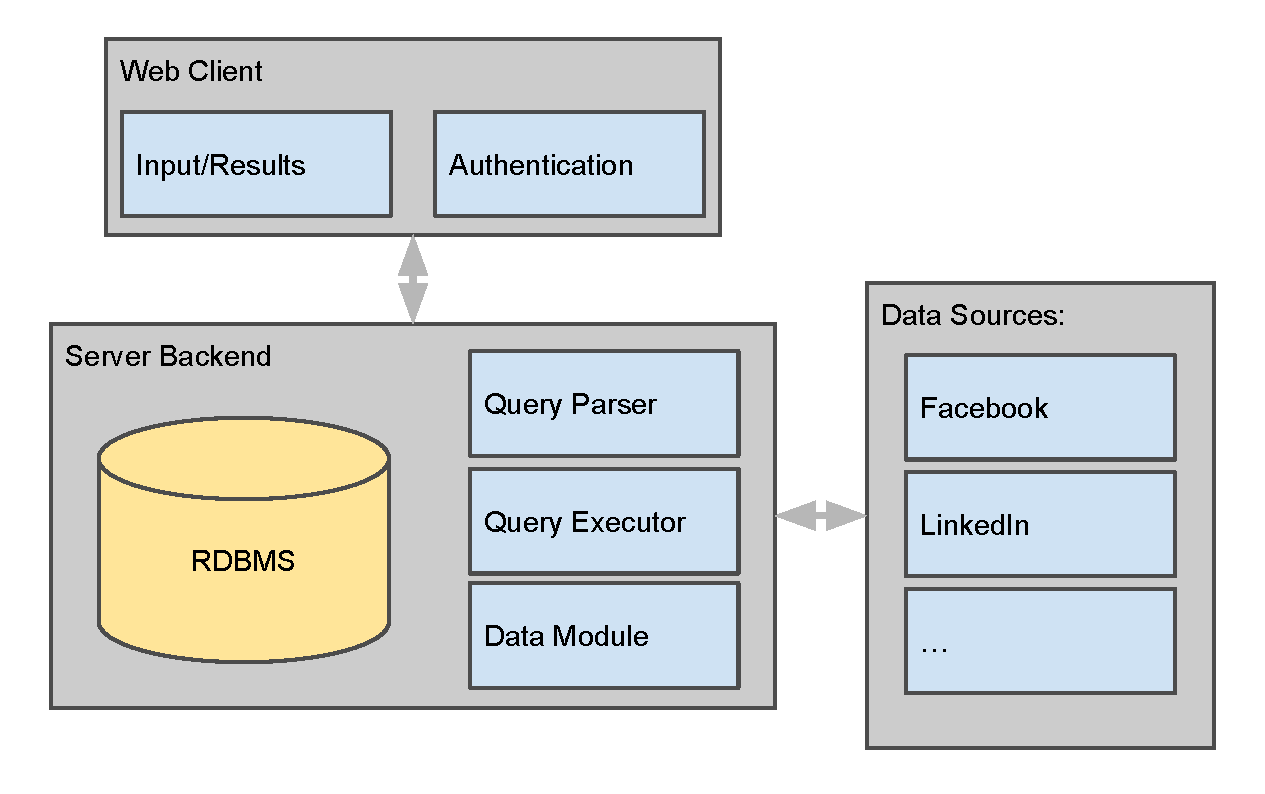
\includegraphics[width=0.75\linewidth]{figs/sysarch.pdf}
\caption{Agent System Architecture}
\label{fig:sysarch}
\end{center}
\end{figure}

Our system architecture is shown in Figure~\ref{fig:sysarch}. At the highest
level, Agent comprises three components, a web client, a server backend, and set
of data sources. We discuss each in turn, with an eye toward demonstrating how
data flows through the system.

\subsection{Web Client}
The web client, as the user-facing component of the application, is responsible
for capturing user input to pass to the server backend  It is implemented as a
series of models and views using the Python Django framework.

\subsubsection{Input/Results}
\todo{Chris of BLi, please fill in once this is done}

\subsubsection{Authentication}
The web client authenticates users by using the Facebook OAuth API. Although the
current implementation of Agent does not persist user information across
sessions and therefore does not have `accounts,' an account would be implemented
by associating a unique user id with a given facebook OAuth token. A user would
then `link' to other data sources (described below) using their corresponding
APIs. These references would be stored in a table that associates each of these
data sources (Facebook included) with the unique user id for the given account.

\subsection{Server Backend}
The server, like the client, is built as part of a Django application. It is
composed of a number of modules, most of which are built into the application
models and others of which are implemented as standalone utilities.

\subsubsection{Query Parser}
The query parser receives text queries from the web client and resolves them
into sets of entities through a term extraction process. At a high level, it
identifies tags by measuring the likelihood that the words in the query co-occur
and whether their co-occurence in the input is `important' (one measure for
determining this is pointwise-mutual information\footnote{See:
http://www.eecis.udel.edu/~trnka/CISC889-11S/lectures/philip-pmi.pdf} Currently,
we rely on the Yahoo Content Analysis API to tag entities~\cite{yahoo_ca}, but
we could use any reasonable term extraction module in order to determine our
final query form. A more complex, customized term extraction algorithm might
improve our results, but this diverges into linguistics and formal semantics, so
we do not pursue this option in our current implementation.  Furthermore, if we
extended Agent's functionality to accept arbitrary questions (rather than
templated questions), a layer of semantic analysis would be necessary. Again, we
see this as more of a linguistics problem, so we leave it as a potential
extension of the current system.

\subsubsection{Query Executor}
The query executer receives a set of entities from the Query Parser and then
generates the database queries necessary to `score' each connection in the
user's social network.  It then returns the $N$ (a user-configurable parameter)
connections with the highest score.  The score corresponds to the likelihood
that the connection might be able to answer the inputed query. Agent's scoring
algorithm and the corresponding SQL are presented in Section~\ref{sec:scoring}.

In our implementation, the SQL is actually generated on-the-fly by the Django
framework. Our interface to the data is therefore through the models API rather
than through the underlying RDBMS.

\subsubsection{Data Module}
The data module is responsible for retrieving data from each of the user's
linked data sources and transforming that data into the end format utilized by
our RDBMS (we call these data {\it interactions}). Agent's data model and ETL
process are detailed in Section~\ref{sec:data}. The module is implemented as a
collection of Python utilities.

\subsubsection{RDBMS}
The RDBMS is responsible for persisting account information (the set of linked
accounts associated with a given user id) as well as the set of interactions for
each connection. These interactions are the target of Agent queries. The RDBMS
therefore interacts with both the Query Executor and Data Module. Agent uses
Postgres as its RDBMS.

\subsection{Data Sources}
The data sources are any social networking sites that define users and
connections among users, along with a profile or set of actions that a user can
perform. In the current implementation, we support Facebook as a data source,
but this is easily extensible to sites such as LinkedIn and Tumblr. Agent
accesses the data sources using the credentials provided during authentication
through the REST APIs offered by each source. For each site, we implement a new
ETL module to transform the data to our target format (described in
Section~\ref{sec:data}).
